\documentclass{beamer}
\usetheme{Singapore}
\usepackage{multicol}
\usepackage{graphicx}
\newcommand{\yellow}{}
%\documentclass[a4paper,azure,pdf,colorBG,slideColor]{prosper}
%\documentclass{prosper}
%\hypersetup{pdfpagemode=FullScreen}


%\usepackage{pstricks,pst-node,pst-tree}

%\setlength{\topmargin}{-0.5in}
%\setlength{\textwidth}{9in}
%\setlength{\oddsidemargin}{-1in}
%\setlength{\evensidemargin}{-1in}

%\newcommand{\ns}[1]{\vfill \end{slide}\begin{slide}{#1}}
\newcommand{\bframe}[1]{\begin{frame}[fragile]{#1}}

\newcommand{\bi}{\begin{itemize}}
%\newcommand{\bd}{\begin{itemize}\tt}
\newcommand{\bd}{\begin{itemize}}
\newcommand{\ii}{\item}
\newcommand{\ei}{\end{itemize}}
%\newcommand{\ed}{\rm\end{itemize}}
\newcommand{\ed}{\end{itemize}}

\newcommand{\sk}{}%{\vspace{0.2in}}


\title{Inform 7 Notes}

\author{Geoffrey Matthews\\\small (Based on the help files.)}


\begin{document}
\begin{frame}
\maketitle
\end{frame}

\bframe{Inform 7 Basic Concepts}
\bi
\item Actions (things the player can do):
\bd \item Take the cat \ed
\item Sentences (things the programmer can do):
\bi
\item Assertions\bd\item The cat is on the mat.\ed
\item Phrases\bd\item Say "Look out!"\ed
\item Rules
\bd\item Instead of taking the cat: \\\ \ \ say "It's claws are too sharp."\ed
\item Relations
\bd\item Every turn:\\\ \ \ if {\bf the cat is on the mat}, say "purr".\ed
\ei
\ei

\end{frame}
\bframe{Example}
\bd
\ii
The switch is a device in the laboratory. \\\ \ 
    "On the wall is a switch, latched firmly \\\ \ 
    in the [if switched on]on[otherwise]off[end if]\\\ \ 
    position."

\ii
After switching on the switch, \\\ \ say "The
    gears begin to turn."
\ii
After switching off the switch, \\\ \ say "The
    room falls quiet."
\ii
Every turn when in the laboratory and the switch is switched on: \\
    say "Gears and chains clank and whirr about you."

\ii

Understand "pull {\yellow [a switched off device]}" as switching on.
\ii
Understand "pull {\yellow [a switched on device]}" as switching off.
\ed

\end{frame}
\bframe{Assertions}
\bd
\ii
The wood-slatted crate is in the Gazebo.  The crate is a container.
\ed

\end{frame}
\bframe{Rules}
\bd
\ii
Instead of taking the crate, say "It's far too heavy to lift." 
\ii
Before taking the crate: \\
\ \ if the player is wearing the hat: \\
\ \ \ \ now the hat is in the crate; \\
\ \ \ \ say "As you stoop down, your hat falls into the crate."
\ed
\end{frame}
\bframe{Descriptions}
\bd
\ii
The Cobble Crawl is a room. "You are crawling over cobbles in a low passage. There is a dim light at the east end of the passage." 

\ii

A wicker cage is here. "There is a small wicker cage discarded nearby." 
\ed
\end{frame}
\bframe{Rooms and the Map}

\bd
\ii
Inside from the Meadow is the woodcutter's hut. 

\ii
The Airport Road is west of the Fish Packing Plant. A room called the Airport is west of the Airport Road. 

\ii
The Debris Room is west of the Crawl.

\ii

East of the Debris Room is nowhere.

\ed
\end{frame}
\bframe{Kinds}

\bd
\ii
East of the Garden is the Gazebo. Above is the Treehouse. A billiards table is in the Gazebo. On it is a trophy cup. A starting pistol is in the cup.
\ed
\bi

\ii
Garden, Gazebo, Treehouse - room 

\ii
billiards table - supporter 

\ii
cup - container 

\ii
starting pistol - thing 
\ii
East, up (implied by "above") - direction 
\ed
\end{frame}
\bframe{Scenery}

\bi
\ii
{This will describe the tree twice:}
\ei
\bd
\ii
The Orchard is a room. "Within this quadrille of pear trees, a single gnarled old oak remains as a memory of centuries past." The gnarled old oak tree is fixed in place in the Orchard. 
\ed

\bi
\ii
{This will not describe the tree a second time:}
\ei
\bd
\ii
The Orchard is a room. "Within this quadrille of pear trees, a single gnarled old oak remains as a memory of centuries past." The gnarled old oak tree is scenery in the Orchard. 
\ed

\end{frame}
\bframe{Doors}
\bd
\ii
The heavy iron grating is east of the Orchard and west of the Undertomb. The grating is a door. 

\ii
The old brass key unlocks the heavy iron grating.
\ed
\end{frame}
\bframe{Devices}
\bd
\ii
The coffin is an openable container in the Undertomb. "[if open]The lid of a plank coffin yawns open.[otherwise]A plank coffin lies upon the dirt floor of the Tomb." 
\ed
\end{frame}
\bframe{Light and Darkness}

\bd
\item The Sinister Cave is a dark room.
\item The flaming torch is in the Sandy Passage.  It is lit.
\ed

\end{frame}
\bframe{Descriptions}
\bd
\item Instead of throwing something at a {\bf
closed openable door}, 
say "Or you could just use the handle like anyone else, of course." 
\item ... something worn by woman who is in a dark room ... 
\item Texture is a kind of value. 
The textures are rough, stubbly and smooth. Everything has a texture. 
\item Definition: A supporter is occupied if something is on it. 
\ed

\end{frame}
\bframe{Basic Actions}
\bd
\item Instead of examining something in the Drawing Room, say 
"Under Lady Bracknell's eye, you feel constrained. Besides, it is only
[a noun]." 
\ed

\end{frame}
\bframe{Change}
\bd
\item After going somewhere:\\
~~~  say "Mary follows";\\
~~~  {\bf now} Mary is in the location;\\
~~~  continue the action.
\ed

\end{frame}
\bframe{Time}
\bd
\item When play begins: change the command prompt to \\
"[time of day] : " \sk
\item Every turn: ... \sk
\item When play ends: ... \sk 
\item At 4 PM: say "The great bells of the clock tower chime four." \sk
\item Instead of waiting when it is after 4:00 PM: ...
\ed

\end{frame}
\bframe{Scenes}
\bi
\ii Used to create action in response to a situation, rather than a
particular action by the player.
\ei
\bd
\item Train Stop is a scene.
\item Train Stop begins when the player is in the Station for the
  third turn. 
\item When Train Stop begins:\\
move the Flying Scotsman to the Station.\\ 
say "The Flying Scotsman pulls up at the platform, billowing steam.
\ed
\end{frame}


\bframe{Phrases}
\bd
\item say "Look out!"\sk
\item now the hat is in the crate\sk
\item move the player to the Well House\sk
\item if the player is holding the amulet, award 20 points\sk
\ed

\end{frame}
\bframe{New Phrases}
\bd
\item To spring the trap:\\
~~~ say "'Sproing!' go the hinges and, with a flash \\
~~~ of silver, the
enormous blades whisk \\ ~~~ together!";  \\
~~~ end the game in death. \sk
\item To slam shut (box - an open container):\\
~~ say "With panache, you slam shut [the box].". 
\sk
\item Instead of closing the box:
~~ slam shut the box.
\ed

\end{frame}
\bframe{Actions Processing}

\centerline{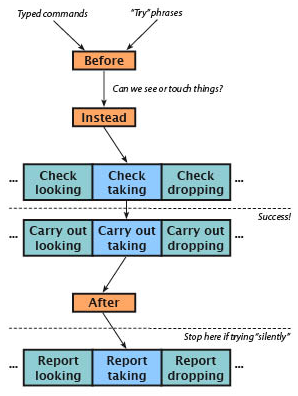
\includegraphics[width=2.25in]{actionschart.png}}


\end{frame}
\bframe{New Actions}
\bd
\item Photographing is an action applying to one visible thing 
and requiring light. \sk
\item Understand "photograph [something]" as photographing. \sk
\item
Check photographing: if we have photographed the noun then say "You've already snapped [the noun]." instead. 
\sk \item
Carry out photographing: now film is film - 1
\sk
\item
Report photographing: say "Click!" 
\ed

\end{frame}
\bframe{Relations}
\bd
\item The mouse {\bf is in} the teapot.
\item ... now the mouse {\bf is in} the teapot ...
\item ... if Mr Darcy {\bf can see} the mouse ...
\item ... things which {\bf are in} the teapot ...
\ed

\end{frame}
\bframe{Inform builtin relations}
\bi

\item containment relation - {\tt The coin is in the purse. }
\item support relation - {\tt The coin is on the table. }
\item incorporation relation - {\tt The coin is part of the sculpture. }
\item carrying relation - {\tt The coin is carried by Peter. }
\item wearing relation - {\tt The jacket is worn by Peter. }
\item possession relation - {\tt if Mr Darcy has a rapier... }
\item adjacency relation - {\tt The Study is east of the Hallway. }
\item visibility relation - {\tt if Darcy can see Elizabeth... }
\item touchability relation - {\tt if Darcy can touch Elizabeth... }

\ei

\end{frame}
\bframe{New relations}

\bd
\item Loving relates various people to one person. 
\item Meeting relates people to each other. 
\item Marriage relates one person to another (called the spouse). 
\item Nationality relates people to each other in groups. 
\ed

\end{frame}
\bframe{New verbs for relations}
\bd
\item The verb to sport (he sports, they sport, he sported, it is sported, he is sporting) implies the wearing relation. 

\ed

\end{frame}
\bframe{New prepositions for relations}
\bd
\item Suspecting relates various people to one person. 
\item The verb to suspect (he suspects, they suspect, he suspected, 
it is suspected, he is suspecting) implies the suspecting relation. 
\item 
The verb to be suspicious of implies the suspecting relation. \sk
\item
Hercule Poirot suspects Colonel Hotchkiss. 
\item
Hercule Poirot is suspicious of Colonel Hotchkiss. \sk
\item
somebody who suspects Colonel Hotchkiss 
\item
somebody suspicious of Colonel Hotchkiss 

\ed


\end{frame}
\bframe{Understanding (grammar)}

\bd
\item Understand "photograph [someone]" as photographing. 
\item Understand "deposit [something] in [an open container]" as
inserting it into. 
\item
Understand "fill [an open container] with [something]" as inserting it into (with nouns reversed).
\item Understand "wear [something held]" as wearing. 
\item Understand "take [things inside] from [something]" as removing. 
\item Understand "put [other things] in/inside/into [something]" as
inserting it into. 
\ed

\end{frame}
\bframe{Understanding (grammar)}

\bd
\item Understand "scarlet" or "crimson" as red.\sk
\item Understand "reach underneath/under/beneath [something]" as
looking 
under. 
\ed

\end{frame}
\bframe{Rules}
\bd
\item Every turn, say "The summer breeze shakes the apple-blossom." \sk
\item This is the blossom shaking rule: say "The summer breeze shakes
the apple-blossom." 
\item The blossom rule is listed in the every turn rules. 
\ed
\end{frame}
\bframe{Procedural rules}
\bd
\item
A procedural rule: if in the Timeless Void then ignore the advance time rule. 
\ed

\end{frame}
\end{document}
 
